\section{Relationen}

\begin{figure}[H]
	\centering
	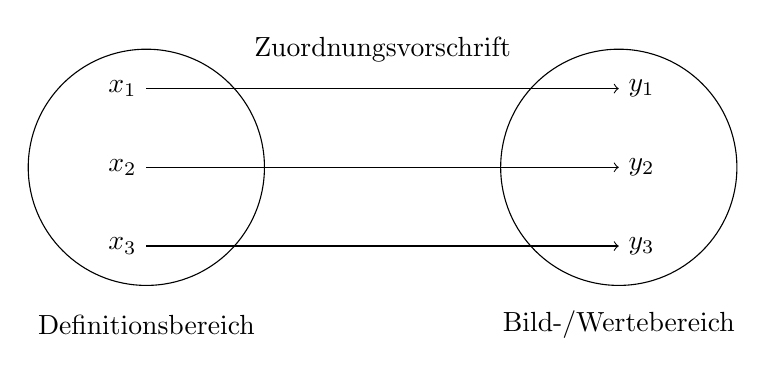
\begin{tikzpicture}
		\draw (0,0) circle (1.5cm);
		\node[left] at (0,1) {\(x_1\)};
		\node[left] at (0,0) {\(x_2\)};
		\node[left] at (0,-1) {\(x_3\)};
		\node at (0,-2) {Definitionsbereich};

		\draw[->] (0, 1) -- (6, 1);
		\draw[->] (0, 0) -- (6, 0);
		\draw[->] (0,-1) -- (6,-1);
		\node at (3,1.5) {Zuordnungsvorschrift};

		\draw (6,0) circle (1.5cm);
		\node[right] at (6,1) {\(y_1\)};
		\node[right] at (6,0) {\(y_2\)};
		\node[right] at (6,-1) {\(y_3\)};
		\node at (6,-2) {Bild-/Wertebereich};
	\end{tikzpicture}
\end{figure}

\[
	R = \{ (x,y) \mid x \in D, y \in B, x\ R\ y \}
\]

mit \(D\) als Definitionsbereich,
\(B\) als Bildbereich und
\(R\) als Zuordnungsvorschrift.

\subsection{Darstellungsformen}

\paragraph{explizite Darstellungsform}

\[
	y = f(x)
\]

\subparagraph{Beispiel}

\[
	y = \sqrt{1-x^2}
\]

\paragraph{implizite Darstellungsform}

\[
	F(x,y) = 0
\]

\subparagraph{Beispiel}

\[
	x^2 + y^2 - 1 = 0
\]

\paragraph{Parameterdarstellung}

\[
	x = x(t)
\]
\[
	y = y(t)
\]

\subparagraph{Beispiel}

\begin{align*}
	x               & = \cos(t)   \\
	\Rightarrow x^2 & = \cos^2(t) \\
	y               & = \sin(t)   \\
	\Rightarrow y^2 & = \sin^2(t)
\end{align*}

\[
	\underbrace{\cos^2(t) + \sin^2(t)}_{\text{Einheitskreis}} = 1 = x^2 + y^2
\]

